\PassOptionsToPackage{unicode=true}{hyperref} % options for packages loaded elsewhere
\PassOptionsToPackage{hyphens}{url}
%
\documentclass[]{article}
\usepackage{lmodern}
\usepackage{amssymb,amsmath}
\usepackage{ifxetex,ifluatex}
\usepackage{fixltx2e} % provides \textsubscript
\ifnum 0\ifxetex 1\fi\ifluatex 1\fi=0 % if pdftex
  \usepackage[T1]{fontenc}
  \usepackage[utf8]{inputenc}
  \usepackage{textcomp} % provides euro and other symbols
\else % if luatex or xelatex
  \usepackage{unicode-math}
  \defaultfontfeatures{Ligatures=TeX,Scale=MatchLowercase}
\fi
% use upquote if available, for straight quotes in verbatim environments
\IfFileExists{upquote.sty}{\usepackage{upquote}}{}
% use microtype if available
\IfFileExists{microtype.sty}{%
\usepackage[]{microtype}
\UseMicrotypeSet[protrusion]{basicmath} % disable protrusion for tt fonts
}{}
\IfFileExists{parskip.sty}{%
\usepackage{parskip}
}{% else
\setlength{\parindent}{0pt}
\setlength{\parskip}{6pt plus 2pt minus 1pt}
}
\usepackage{hyperref}
\hypersetup{
            pdftitle={Analisis de Variables predictoras},
            pdfauthor={Sebastian Jaremczuk},
            pdfborder={0 0 0},
            breaklinks=true}
\urlstyle{same}  % don't use monospace font for urls
\usepackage[margin=1in]{geometry}
\usepackage{listings}
\newcommand{\passthrough}[1]{#1}
\usepackage{graphicx,grffile}
\makeatletter
\def\maxwidth{\ifdim\Gin@nat@width>\linewidth\linewidth\else\Gin@nat@width\fi}
\def\maxheight{\ifdim\Gin@nat@height>\textheight\textheight\else\Gin@nat@height\fi}
\makeatother
% Scale images if necessary, so that they will not overflow the page
% margins by default, and it is still possible to overwrite the defaults
% using explicit options in \includegraphics[width, height, ...]{}
\setkeys{Gin}{width=\maxwidth,height=\maxheight,keepaspectratio}
\setlength{\emergencystretch}{3em}  % prevent overfull lines
\providecommand{\tightlist}{%
  \setlength{\itemsep}{0pt}\setlength{\parskip}{0pt}}
\setcounter{secnumdepth}{0}
% Redefines (sub)paragraphs to behave more like sections
\ifx\paragraph\undefined\else
\let\oldparagraph\paragraph
\renewcommand{\paragraph}[1]{\oldparagraph{#1}\mbox{}}
\fi
\ifx\subparagraph\undefined\else
\let\oldsubparagraph\subparagraph
\renewcommand{\subparagraph}[1]{\oldsubparagraph{#1}\mbox{}}
\fi

% set default figure placement to htbp
\makeatletter
\def\fps@figure{htbp}
\makeatother

\usepackage{booktabs}
\usepackage{longtable}
\usepackage{array}
\usepackage{multirow}
\usepackage{wrapfig}
\usepackage{float}
\usepackage{colortbl}
\usepackage{pdflscape}
\usepackage{tabu}
\usepackage{threeparttable}
\usepackage{threeparttablex}
\usepackage[normalem]{ulem}
\usepackage{makecell}
\usepackage{xcolor}

\title{Analisis de Variables predictoras}
\author{Sebastian Jaremczuk}
\date{2020-04-17}

\begin{document}
\maketitle

\hypertarget{carga-de-datos}{%
\subsubsection{carga de datos}\label{carga-de-datos}}

\begin{lstlisting}
## 
## Recursive feature selection
## 
## Outer resampling method: Bootstrapped (10 reps) 
## 
## Resampling performance over subset size:
## 
##  Variables Accuracy  Kappa AccuracySD KappaSD Selected
##          2   0.8002 0.5775   0.009438 0.01841         
##          3   0.8057 0.5894   0.007854 0.01437         
##          4   0.8108 0.6097   0.007263 0.01542         
##          5   0.8138 0.6160   0.008519 0.01816         
##          6   0.8305 0.6518   0.007395 0.01326         
##          7   0.8326 0.6558   0.009898 0.01908         
##          8   0.8353 0.6618   0.009230 0.01785         
##          9   0.8378 0.6670   0.007629 0.01511         
##         10   0.8389 0.6691   0.008728 0.01706        *
##         11   0.8382 0.6679   0.007608 0.01454         
##         12   0.8354 0.6621   0.006773 0.01246         
##         13   0.8347 0.6609   0.009685 0.01884         
##         14   0.8347 0.6608   0.010062 0.01914         
##         15   0.8361 0.6637   0.012528 0.02461         
##         16   0.8335 0.6584   0.009853 0.01902         
##         17   0.8381 0.6678   0.010261 0.02082         
##         18   0.8386 0.6688   0.011634 0.02245         
##         19   0.8381 0.6679   0.012168 0.02348         
##         20   0.8361 0.6636   0.010543 0.02107         
##         21   0.8348 0.6611   0.011929 0.02357         
##         22   0.8355 0.6625   0.013509 0.02702         
##         23   0.8369 0.6655   0.013347 0.02625         
##         24   0.8345 0.6605   0.012766 0.02547         
## 
## The top 5 variables (out of 10):
##    ciclo_lectivo_de_cursada, tipo_de_aprobacion_libre, Turno_Noche, tipo_de_aprobacion_no_firmo, Aprobado
\end{lstlisting}

\begin{lstlisting}
##  [1] "ciclo_lectivo_de_cursada"    "tipo_de_aprobacion_libre"   
##  [3] "Turno_Noche"                 "tipo_de_aprobacion_no_firmo"
##  [5] "Aprobado"                    "Turno_Tarde"                
##  [7] "Nota_max_prom"               "tipo_de_aprobacion_firmo"   
##  [9] "Turno_Manana"                "cant_resursada_regular"
\end{lstlisting}

\begin{table}[!h]

\caption{\label{tab:top_10_rfe_accuracy}Top 10 Modelos con cantidad de variables seleccionadas según Accuracy}
\centering
\begin{tabular}[t]{rrr}
\toprule
\rowcolor{black}  \multicolumn{1}{c}{\textcolor{white}{\textbf{Variables}}} & \multicolumn{1}{c}{\textcolor{white}{\textbf{media\_accuracy}}} & \multicolumn{1}{c}{\textcolor{white}{\textbf{media\_kappa}}}\\
\midrule
\rowcolor{gray!6}  10 & 0.8388631 & 0.6690887\\
18 & 0.8385668 & 0.6687514\\
\rowcolor{gray!6}  11 & 0.8381883 & 0.6678640\\
19 & 0.8381476 & 0.6679149\\
\rowcolor{gray!6}  17 & 0.8380654 & 0.6677621\\
\addlinespace
9 & 0.8377655 & 0.6670357\\
\rowcolor{gray!6}  23 & 0.8368520 & 0.6655250\\
20 & 0.8360972 & 0.6636373\\
\rowcolor{gray!6}  15 & 0.8360919 & 0.6637290\\
22 & 0.8355010 & 0.6625480\\
\bottomrule
\end{tabular}
\end{table}

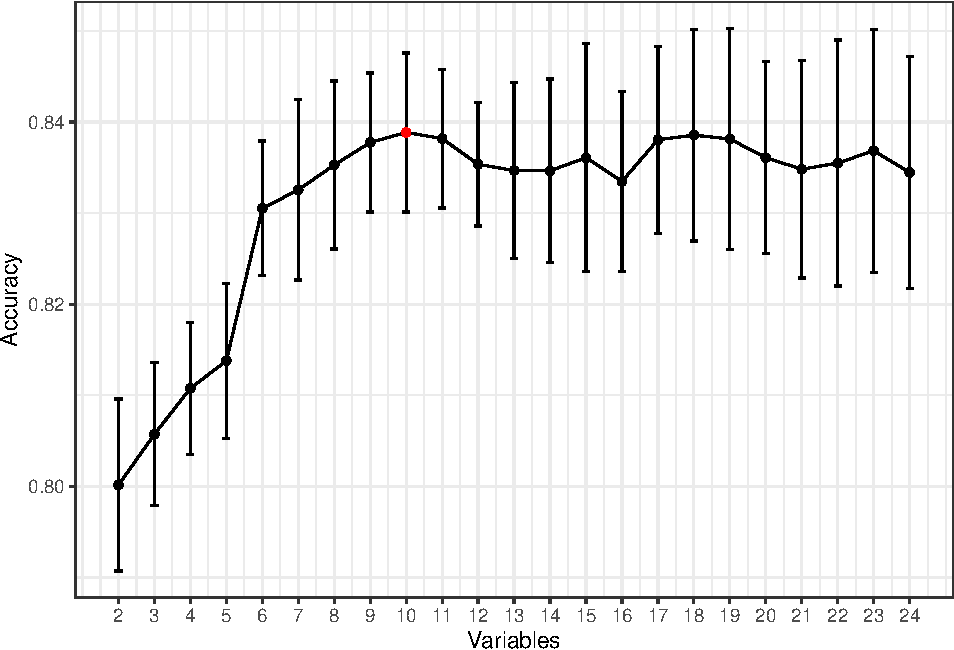
\includegraphics{analisis_de_variables_files/figure-latex/rfe_evolucion_accuracy-1.pdf}

El mejor resultado se consigue con modelos que tienen las 10 variables
mencionadas anteiormente y en el grafico puede verse la evolución de
dich métrica en función de la cantidad de varables que usa con su
dispersión según todos los modelos generados con esa combinación.

tras ajustar cada modelo, se recalcula la influencia de cada variable.
De esta forma, para cada tamaño de modelo, se obtiene un ranking de la
importancia promedio de las variables.

\begin{table}[!h]

\caption{\label{tab:tf_rfe_influencia_variables}Influencia de variables en el resultado}
\centering
\begin{tabular}[t]{lrr}
\toprule
\rowcolor{black}  \multicolumn{1}{c}{\textcolor{white}{\textbf{var}}} & \multicolumn{1}{c}{\textcolor{white}{\textbf{media\_influencia}}} & \multicolumn{1}{c}{\textcolor{white}{\textbf{sd\_influencia}}}\\
\midrule
\rowcolor{gray!6}  ciclo\_lectivo\_de\_cursada & 89.84029 & 2.9668673\\
tipo\_de\_aprobacion\_libre & 46.34285 & 2.2575528\\
\rowcolor{gray!6}  Turno\_Noche & 38.07504 & 1.7175035\\
tipo\_de\_aprobacion\_no\_firmo & 38.05189 & 1.5399760\\
\rowcolor{gray!6}  Aprobado & 35.80734 & 1.1307306\\
\addlinespace
Turno\_Tarde & 35.67467 & 1.5035133\\
\rowcolor{gray!6}  tipo\_de\_aprobacion\_firmo & 35.28770 & 0.6960169\\
Nota\_max\_prom & 35.14407 & 2.3991503\\
\rowcolor{gray!6}  Turno\_Manana & 34.30645 & 1.5999039\\
cant\_resursada\_regular & 32.25476 & 1.1929776\\
\addlinespace
\rowcolor{gray!6}  edad\_al\_ingreso & 31.90459 & 0.1024266\\
\bottomrule
\end{tabular}
\end{table}

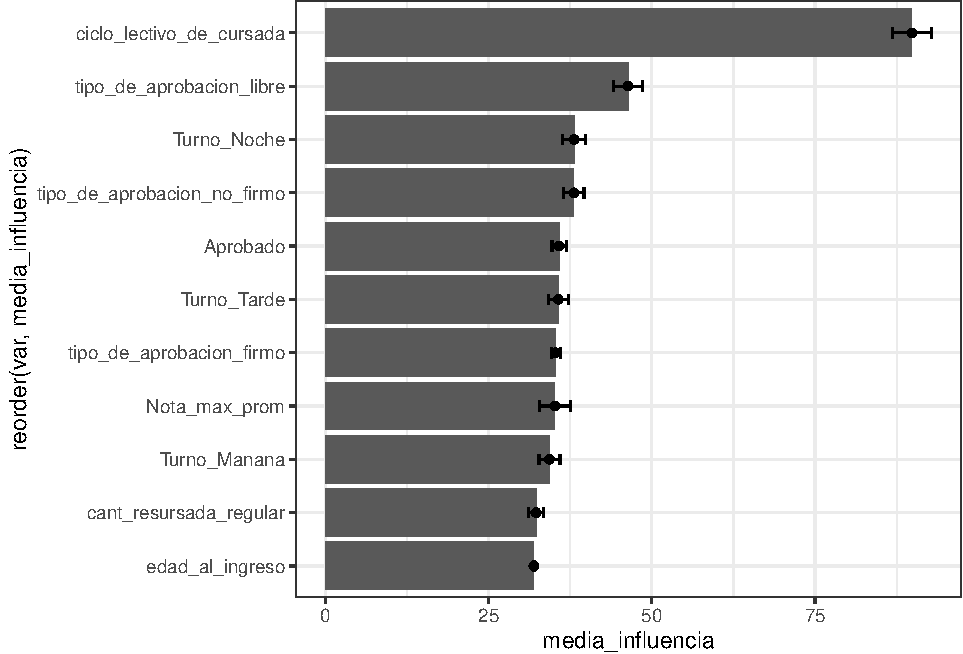
\includegraphics{analisis_de_variables_files/figure-latex/influencia_de_variables-1.pdf}

Existe una variable que claramente influye mucho mas en los resultados
que los otros predictores.

\end{document}
